% !TEX root = holder_flie.tex

\chapter{Monte Carlo Method: Monte Carlo Method and Option Pricing}
%%

\section{Monte Carlo Method}
\noindent The Monte Carlo Simulation, which uses a large number of random numbers, may prove to be a better alternative when there is a high level of uncertainty for estimating or predicting, as opposed to just replacing the uncertain variable with a single average number.\\[2mm]
For processes that are difficult to forecast because of the involvement of random variables, Monte Carlo methods are used to model the likelihood of various outcomes. It is a method for comprehending how risk and uncertainty affect forecasting and prediction models.
\section{Monte Carlo Simulation History}
Since chance and random results are essential to the modeling technique, just as they are to games like roulette, dice, and slot machines, Monte Carlo simulations are called after the well-known gambling location in Monaco.
Stanislaw Ulam, a mathematician who worked on the Manhattan Project, invented the method initially. Ulam kept himself occupied after the war while he recovered from brain surgery by playing endless rounds of solitaire. He developed an interest in graphing the results of each of these games so that he could examine their distribution and calculate the likelihood of winning. John Von Neumann and he worked together to create the Monte Carlo simulation after sharing their concept.
\section{History of Monte Carlo in Finance}
David B. Hertz published an essay in the Harvard Business Review in 1964 outlining the use of Monte Carlo methods in corporate finance, which was the first to bring them to the attention of the finance industry. Phelim Boyle was the first to employ simulation in the valuation of derivatives in his key Journal of Financial Economics work from 1977.\\[2mm]

%%\ref{https://www.youtube.com/channel/UCUcpVoi5KkJmnE3bvEhHR0Q}


\section{A Practical Example with Code}
\noindent Dart problem is a nice illustration for best comprehending the Monte Carlo approach. In this issue, we'll assume that there is a square with side 2 units, and that there is a circle with radius 1 units inside the square. Now that we know the probability of striking the circle if we toss a dart into the square, we must throw the dart at random.\\[2mm]

Therefore, on a 2-D plane with a domain defined as a square with a side of 2 units and centered on (0,0). Imagine a circle with the same radius as the square—one unit—within the same domain. The ratio between the number of points inside the circle and the overall number of points generated is then determined. \\
the area of that circle is $C=\pi$ \\
the area of that square is $S=4$ \\
the ratio would be
$\frac{C}{S}=\frac{\pi}{4}=\frac{\text{no. of points in }C}{\text{no. of points in }S}$\\[2mm]

we have to generate some random numbers for (x, y) then test it if it satisfies the following inequality 
$$x^2+y^2<=1$$. 


However, the frequency interpretation of probability informs us that as the number of trials rises, the approximation becomes more precise. Let's increase the number of trials and plot the results to see why this is the case. I ran simulations between 100 and 1000 times. Below is a display of the simulations' outcomes.\\

\subsection{Convergence of Monte Carlo}
\begin{figure}[H]
	\begin{center}
		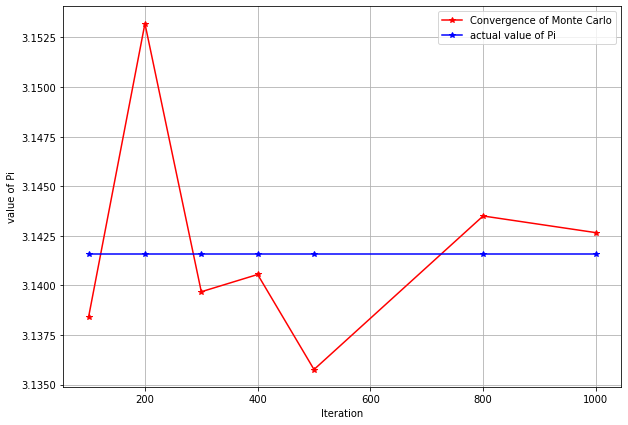
\includegraphics[width=0.8\textwidth]{dart_prob}
	\end{center}
	\caption{Convergence of Monte Carlo}
\end{figure}

\noindent From this graph we can say that MC method can converge to its actual value if we increase the number of iteration. 

\begin{table}[H]
	\begin{center}
		\begin{NiceTabular}{|c|c|c|}[hvlines]
			\rowcolor{blue!20} Serial No. & Interval & Output  \\ 
			1 & 100 & 3.1384 \\
			2 & 200 & 3.1532 \\
			3 & 300 & 3.13968 \\
			4 & 400 & 3.14055 \\
			5 & 500 & 3.13576  \\ 
			6 & 800 & 3.1435  \\ 
			7 & 1000 & 3.14266  \\
			
		\end{NiceTabular}
	\end{center}
	\caption{Monte Carlo Method for Dart Problem}
\end{table}
%\url{https://colab.research.google.com/drive/1VQ95AiamlMWGvvWfpMmaV1nH_NNBiNgG?usp=sharing}


\sect{\section{Option Pricing}}
\noindent We assess analytical solutions known as "vanilla options" for the most fundamental scenarios, such as European puts and calls. These equations are the first and most often used because they are simple to employ, sometimes even in situations when they are not quite appropriate. Contrarily, Monte Carlo is always appropriate, even though in some circumstances the solution calls for considerable dexterity. One of these occurs when future knowledge is required to make judgments in the present. It holds true for American choices. We'll look at how simulation can help tackle the problem of advanced knowledge.

The bulk of non-vanilla possibilities, however, are only path-dependent, do not call for expert knowledge, and are easily managed. We must first think about the standard scenario before we investigate unconventional solutions. It is simple to value the option at the ending price ST, discount the value back to time 0, and value the option if the option's price is not path dependent. The option's price is determined by averaging these values across a sufficient number of samples because this is only one sample.

\sub{\subsection{Monte Carlo as a tool for Financial Math}}
\noindent We'll learn more about the Monte Carlo simulation technique for pricing financial derivatives right now. Only by employing the financial mathematics of risk-neutral pricing and modeling risk-neutral asset pathways is the valuation of financial derivatives through Monte Carlo simulations conceivable.\\
\begin{equation}
	\frac{C_{t}}{B_{t}}= E_{Q}[\frac{C_{T}}{B_{T}}|F_{t}]
\end{equation}
\sub{\subsection{Computationally inefficient}}
\noindent In its most fundamental form, Monte Carlo is inefficient when compared to the straightforward mathematical equations that are available for some deterministic PDEs, such as the Black-Scholes option pricing model for European Options. The method for pricing sophisticated derivatives is, of course, the main factor in our decision to choose Monte Carlo.

In any case, we can improve the accuracy by using:
\begin{itemize}
	\item Antithetic Variates.\\[-2mm]
	\item Control Variates
\end{itemize}
\sub{\subsection{Valuation by Simulation}}
\noindent According to the method of risk-neutral pricing, an option's value equals the risk-neutral expectation of its discounted payment.
By calculating the mean of many deferred payoffs, we can estimate this expectation. Regarding a certain simulation, i:

\begin{equation}
	C_{0,i}= C_{T,i}e^{\int_{0}^{T}-r_{s}\,ds}\\
\end{equation}
\begin{equation}
	C_{0,i}=e^{-rT}C_{T,i}
\end{equation}

\noindent Now if we repeat the simulation M times, we can average the outcomes.\\
\begin{equation}
	\hat{C}_{0}=\frac{1}{M} \sum_{i=1}^{M} C_{0,i}
\end{equation}
\noindent \^{C} is an estimate of the true value of the option 
C\textsubscript{0} with error due to the fact we are taking an average of randomly generated samples, and so therefore the calculation is itself random. A measure of this error is the standard deviation of 
\^{C} called the standard error. This can be estimated as the standard deviation of C\textsubscript{0,i} divided by the number of samples M.
$$SE(\hat{C}_{0})=\frac{\sigma(C_{0,i})}{\sqrt{M}}$$ 

%$${\sigma(C_{0,i})}=\sqrt{\frac{1}{M-1}\[ \sum_{i=1}^{M} (C_{0,i}-\hat{C_{0}})^2\]}}$$
\sub{\subsection{European Call Option in the Black-Scholes World}}
\noindent Here we have constant interest rate so the discount factor is exp(-rT) and the stock dynamics are modelled with Geometric Brownian Motion GBM.
$$dS_{t}=rS_{t}dt+\sigma S_{t}dW_{t}$$
Let’s simulate this GBM process by simulating variables of the natural logarithm process of the stock price
$$x_{t}=ln(S_{t})$$ 
which is normally distributed. For the dynamics of the natural logarithm process of stock prices under GBM model we need to use Ito’s calculus.
$$dx_{t}=vdt+\sigma dz_{t}$$
$$v=r-\frac{1}{2}\sigma^2$$
We can then discretize the Stochastic Differential Equation SDE by changing the infinitesimals dx,dt,dz into small steps $\Delta x$,$\Delta t$,$\Delta z$
$$\Delta x=v\Delta t+\sigma\Delta z$$
This is the exact solution to the SDE and involves no approximation.
$$x_{t+\Delta t}=x_{t}+v\Delta t+\sigma(z_{t+\Delta t}-z_{t})$$
In terms of the stock price S, we have:
$$S_{t+\Delta t}=S_{t}\exp({v\Delta t+\sigma(z_{t+\Delta t}-z_{t})})$$
Where
$$(z_{t+\Delta t}-z_{t}) \sim N(0,\Delta t)\sim \sqrt{\Delta t}N(0,1) \sim \sqrt{\Delta t}\epsilon_{i}$$

\sub{\subsection{Algorithm}} 
\noindent Monte Carlo continuous pricing algorithm\\
inputs:  \\
$S, K, vol, r, N, M, T$ \newline
Steps:
$dt=T/N$ \newline
$nudt=(r-0.5vol^2)*dt$  \newline
$volsdt=volsqrt(dt)$  \newline
$sumCT=0$  \newline
$sumCT2=0$  \newline
\indent $lnSt=lnSt+nudt+volsdt*epsilon$  \newline
\indent $ST=exp(lnSt)$  \newline
\indent $CT=max(0,ST-k)$  \newline
\indent $sumCT=sumCT+CT$  \newline
\indent $sumCT=sumCT2+CT*CT$  \newline
$C0=exp(-rT)sumCT/M$  \newline


\sub{\subsection{Result}}

\begin{center}
	\begin{NiceTabular}{|c|c|c|c|}[hvlines]
		\rowcolor{blue!20} Maturity & Strike Price & Option Price & Standard Error\\ 
		\Block{7-1}{1} & \Block{7-1}{100} & 3.83 & 0.11 \\ 
		& & 3.65 & 0.11 \\
		& & 3.73 & 0.12 \\
		& & 3.53 & 0.1  \\
		& & 3.77 & 0.11 \\
		& & 3.88 & 0.11 \\
		& & 3.84 & 0.11 \\
	\end{NiceTabular}
\end{center}

\noindent Applying monte carlo method we can see a slide deviation from its actual value. Moreover, the standard error is on average 0.11.

\sub{\subsection{Option Price with Maturity}}

\begin{center}
	\begin{NiceTabular}{|c|c|}[hvlines]
		\rowcolor{blue!20} Maturity & Option Price\\ 
		0.01 & 3.11 \\ 
		0.02 & 3.09 \\
		0.03 & 3.17 \\
		0.04 & 3.15  \\
		0.05 & 3.17 \\
		0.06 & 3.29 \\
		0.07 & 3.33 \\
	\end{NiceTabular}
\end{center}
\noindent Keeping the strike price same we have made this table of maturity and option price. Here, we can see a linear relationship between these two factors. 
\begin{figure}[H]
	\begin{center}
		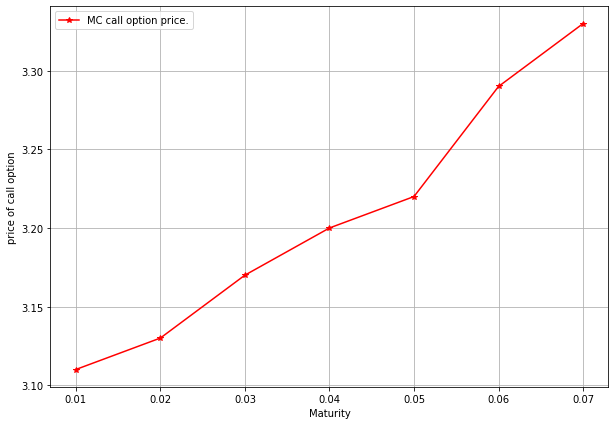
\includegraphics[width=0.8\textwidth]{MC_call_option_price}
	\end{center}
	\caption{Option Price with Maturity}
\end{figure}



\sub{\subsection{Relation Between Option Price and Strike Price}}

\begin{center}
	\begin{NiceTabular}{|c|c|}[hvlines]
		\rowcolor{blue!20} Strike Price & Option Price\\ 
		60 & 41.22 \\ 
		70 & 31.14 \\
		80 & 21.25 \\
		90 & 11.23  \\
		100 & 1.76 \\
	\end{NiceTabular}
\end{center}


\begin{figure}[H]
	\begin{center}
		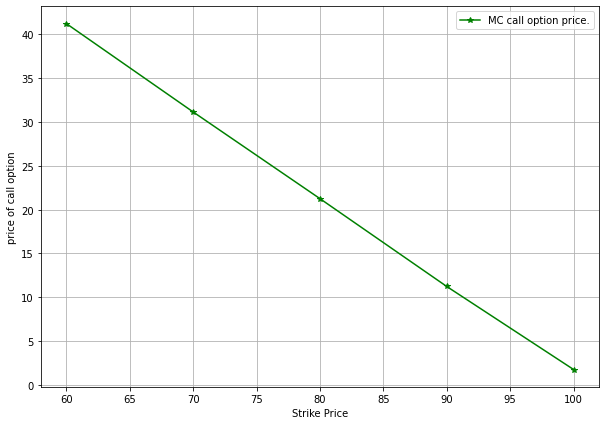
\includegraphics[width=0.8\textwidth]{MC_Strike_Price}
	\end{center}
	\caption{Relation Between Option Price and Strike Price}
\end{figure}
\sub{\subsection{Monte Carlo Variance Reduction Methods – Antithetic}}
\noindent We will now come up with a concept for lowering the variance of the Monte Carlo simulation method while valuing financial derivatives. Unfortunately, while being a fantastic strategy for estimating option values with complex payoffs or high dimensionality, we must run a lot of simulations M in order to obtain an acceptable level of accuracy. Instead, we can rely on strategies for variance reduction, which follow the same rules as hedging an option position. i.e., a hedged option portfolio's volatility will be lower than that of its unhedged equivalent.
\sub{\subsection{Antithetic Variates}}
\noindent Let’s write an option on asset $S_{1}$
and another option on asset $S_{1}$
that is perfectly negatively correlated with $S_{1}$ and which currently has the same price. $S_{1}$
and $S_{2}$ satisfy the following Stochastic Differential Equations:
$$dS_{1,t}=rdS_{1,t}dt+\sigma dS_{1,t}dz_{t}$$
$$dS_{2,t}=rdS_{2,t}dt+\sigma dS_{2,t}dz_{t}$$
The value of these two options is equal because the two assets' prices and volatilities are the same. The volatility of the pay-off of a portfolio that includes both of these contracts, however, is substantially lower than the variance of the pay-off of each contract separately. We are essentially reducing the significant peak in the probability distribution associated with a single contract pay-off. Basic Intuition, i.e., the idea that when one choice succeeds, the other does not.
\sub{\subsection{Implementation of Antithetic Variate}}
\noindent We generate a fictitious asset that is perfectly negatively linked with the real asset in order to apply an antithetic variate. The process of implementation is quite straightforward, and if we use the European Call Option as an example, our simulated pay-offs fall under the following categories: 
$$S_{t+\Delta t}=S_{t}\exp(v\Delta t+\sigma(z_{t+\Delta t}-z_{t}))$$
Where
$$(z_{t+\Delta t}-z_{t}) \sim N(0,\Delta t)\sim \sqrt{\Delta t}N(0,1) \sim \sqrt{\Delta t}\epsilon_{i}$$

\noindent Contract Simulation
$$-C_{T,i}=max(0,S \exp(v\Delta T+\sigma\sqrt{T}(\epsilon_{i}))-K)$$
$$-\bar{C}_{T,i}=max(0,S \exp(v\Delta T+\sigma\sqrt{T}(-\epsilon_{i}))-K)$$
\sub{\subsection{Algorithm}} 
\noindent Monte Carlo continuous pricing algorithm\\
inputs:  \\
$S, K, vol, r, N, M, T$ \newline
Steps:
$dt=T/N$ \newline
$\nu dt=(r-0.5vol^2)*dt$  \newline
$volsdt=volsqrt(dt)$  \newline
$sumCT=0$  \newline
$sumCT2=0$  \newline
\indent $lnSt=lnSt+nudt+volsdt*epsilon$  \newline
\indent $ST=exp(lnSt)$  \newline
\indent $CT=max(0,ST-k)$  \newline
\indent $sumCT=sumCT+CT$  \newline
\indent $sumCT=sumCT2+CT*CT$  \newline
$C0=exp(-rT)sumCT/M$  \newline
\sub{\subsection{Result}}

\begin{center}
\begin{NiceTabular}{|c|c|c|}[hvlines]
	\rowcolor{blue!20} Option Price & SE & Computation Time\\ 
	7.47 & 0.324 & 0.4867\\ 
	7.97 & 0.331 & 0.4845\\
	7.63 & 0.334 & 0.4916\\
\end{NiceTabular}
\end{center}


\sub{\subsection{Option Price with Strike Price}}

\begin{center}
	\begin{NiceTabular}{|c|c|}[hvlines]
		\rowcolor{blue!20} Strike Price & Option Price\\ 
		60 & 41.2 \\ 
		70 & 31.21 \\
		80 & 21.23 \\
		90 & 11.23  \\
		100 & 1.73 \\
	\end{NiceTabular}
\end{center}

\begin{figure}[H]
	\begin{center}
		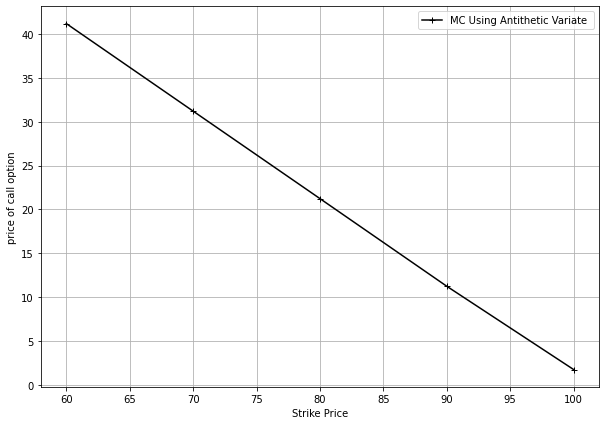
\includegraphics[width=0.8\textwidth]{mc_antithetic}
	\end{center}
	\caption{Option Price with Strike Price}
\end{figure}

\sub{\subsection{Pricing an Up-and-Out Barrier Option}}
\sub{\subsection{Path-Dependent option}}
\noindent The barrier option is a well-liked product when pricing complex or exotic path dependant options. These options have a conventional European option expiration style, but they only become active if the underlying price reaches a predetermined barrier threshold. This barrier level may be monitored continuously or intermittently. $\tau$
For an up-and-out barrier put option:
$$C_{T}=f(S_{T})=(K-S_{T})^+ind( max S_{t}<H)$$

\sub{\subsection{Algorithm}}
\noindent Monte Carlo continuous pricing algorithm\\
inputs:  \\
$S0, K, H, vol, r, N, M, T$ \newline
Steps:
$dt=T/N$ \newline
$\nu dt=(r-0.5vol^2)*dt$  \newline
$volsdt=volsqrt(dt)$  \newline
$sumCT=0$  \newline
$sumCT2=0$  \newline
For $i:$  \newline
\indent $BARIER= FALSE$ \newline
\indent $St=S0$ \newline
\indent For $j:$ \newline
\indent\indent $lnSt=lnSt+nudt+volsdt*epsilon$  \newline
\indent\indent $ST=exp(lnSt)$  \newline
\indent\indent $CT=max(0,ST-k)$  \newline
\indent\indent $sumCT=sumCT+CT$  \newline
\indent\indent $sumCT=sumCT2+CT*CT$  \newline
\indent\indent if BARRIER: \newline
\indent\indent\indent CT=0 \newline
\indent\indent else: \newline
\indent\indent\indent $CT=max(0,K-St)$ \newline
$C0=exp(-rT)sumCT/M$  \newline
\sub{\subsection{Result}}


\begin{center}
\begin{NiceTabular}{|c|c|c|}[hvlines]
	\rowcolor{blue!20} Option Price & SE & Computation Time\\ 
	7.47 & 0.324 & 0.4867\\ 
	7.97 & 0.331 & 0.4845\\
	7.63 & 0.334 & 0.4916\\
\end{NiceTabular}
\end{center}

\sub{\subsection{Option Price with Maturity}}

\begin{center}
	\begin{NiceTabular}{|c|c|}[hvlines]
		\rowcolor{blue!20} Maturity & Option Price\\ 
		0.01 & 0.7 \\ 
		0.02 & 1.09 \\
		0.03 & 1.55 \\
		0.04 & 1.56  \\
		0.05 & 1.76 \\
		0.06 & 2 \\
		0.07 & 1.91 \\
	\end{NiceTabular}
\end{center}

\begin{figure}[H]
	\begin{center}
		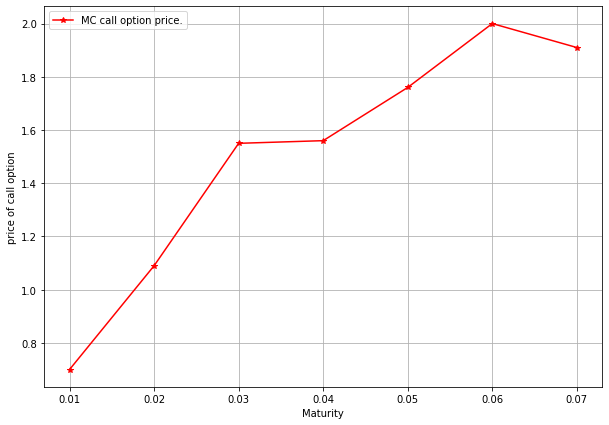
\includegraphics[width=0.8\textwidth]{MC_Barrier_Option_With_Maturity}
	\end{center}
	\caption{Option Price with Maturity}
\end{figure}

\sub{\subsection{Relation Between Option Price and Strike Price}}

\begin{center}
	\begin{NiceTabular}{|c|c|}[hvlines]
		\rowcolor{blue!20} Strike Price & Option Price\\ 
		100 & 1.88 \\ 
		110 & 10.15 \\
		120 & 19.87 \\
		130 & 30.01  \\
		140 & 40.06 \\
	\end{NiceTabular}
\end{center}

\begin{figure}[H]
	\begin{center}
		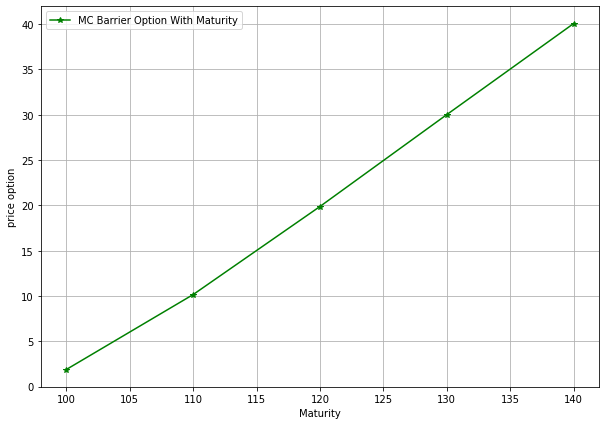
\includegraphics[width=0.8\textwidth]{MC_Barrier_Option_With_Strike_Price}
	\end{center}
	\caption{Option Price and Strike Price}
\end{figure}


\sub{\subsection{The Monte Carlo Method for American Options}}
\noindent As we've seen, the fundamental binomial approach can calculate American option pricing with just a simple and minor change. This is due to the fact that the backward technique works by first determining option prices at expiration and then working backwards to the beginning date. As a result, every time an early exercise is an option, it is simple to decide not to exercise because it is known what the option's future value will be if it is not. Furthermore, there are only two potential outcomes for the future value in question.
A forward technique, however, lacks this kind of future knowledge. Think about the challenge a GRW will face when the option is well-positioned to win at some point in the walk. Even if the discounted expiration value of the option were known at that point, for instance by applying the Black-Scholes formula, the knowledge would not be adequate because there might be additional opportunities for early exercise before expiration. As a result, the option's discounted expiration value does not appropriately reflect its value at the time in question.
However, there is a zone in which, depending on the amount of time left before expiration, the option should be exercised early if it were sufficiently deep in the money. The idea of an exercise boundary is derived from this one.

\sub{\subsection{Algorithm}} 
\noindent Monte Carlo continuous pricing algorithm\\
inputs:  \\
$S_0,T,k, r,\Delta t, \sigma, N$ and the exercise boundary B(t) \newline
$E=0$\\
$n=T/\Delta t$\\
for $i=1,...N$  \newline
\indent $S=S_{0}$\\
\indent for $t=\Delta t,2\Delta t,...n\Delta t$\\
\indent $Z \sim N(0,1)$  \newline
\indent $S_{t}=S_{t-1}(1+rt+\sigma\sqrt{\Delta t}Z)$\\ %\newline
\indent \indent if $K-S_{t}>=KB(T-t)$\\
\indent \indent \indent $E=E+\exp(-rT)(k-S_{t})$ \\ 
\indent \indent \indent go to next i\\
\indent\indent endif\\
\indent end for t
\indent $E=E+\exp(-rT)(k-S_{t})$ \\ 
end for i\\
$E=\frac{E}{N}$ \newline
option price=$\exp(-rT)E$  \newline


\begin{center}
	\begin{NiceTabular}{|c|c|c|c|c|}[hvlines]
		\rowcolor{cyan!20} T & K & European Option & American Option & SE \\ 
		\Block{9-1}{1}& 80 &   0.6812 &   0.6886 &   0.0108 \\
		& 85 &   1.3607 &   1.3657 &   0.0037 \\ 
		& 90 &   2.3019 &   2.4913 &   0.0823 \\
		& 95 &   3.7361 &   3.9601 &   0.0600 \\
		& 100 &   5.6507 &   6.0940 &   0.0784 \\
		& 105 &   7.8782 &   8.7486 &   0.1105 \\
		& 110 &  10.6292 &  11.9784 &   0.1269 \\
		& 115 &  13.6376 &  15.7496 &   0.1549 \\
		& 120 &  17.2459 &  20.1122 &   0.1662 \\
	\end{NiceTabular}
\end{center}

\begin{figure}[H]
	\begin{center}
		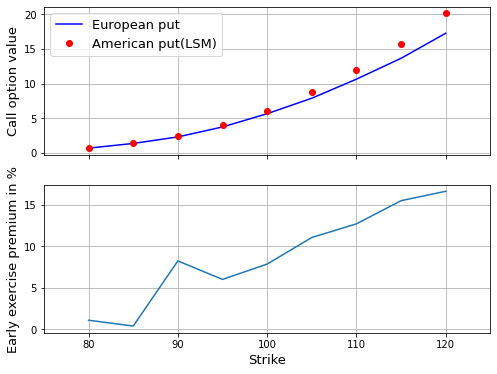
\includegraphics[width=0.8\textwidth]{American_option}
	\end{center}
	\caption{American Put Option}
\end{figure}